\documentclass[conference]{IEEEtran}
\IEEEoverridecommandlockouts
\usepackage{cite}
\usepackage{amsmath,amssymb,amsfonts}
\usepackage{graphicx}
\usepackage{booktabs}
\usepackage{multirow}
\usepackage{textcomp}
\usepackage{xcolor}
\usepackage{hyperref}
\usepackage{caption}
\captionsetup{font=small}

\def\BibTeX{{\rm B\kern-.05em{\sc i\kern-.025em b}\kern-.08em
    T\kern-.1667em\lower.7ex\hbox{E}\kern-.125emX}}

\begin{document}

\title{From Categorization to Resolution: A Comparative Evaluation of a Retrieval-Augmented, Judge-Evaluated LLM Pipeline Against Classical NLP Ticket Classification}

\author{
\IEEEauthorblockN{Ranuga Weerasekara}
\IEEEauthorblockA{Clario \\ ranugaweerasekara2@gmail.com}
\and
\IEEEauthorblockN{Sineth Wickramaratna}
\IEEEauthorblockA{Clario}
}

\maketitle

\begin{abstract}
Customer support ticket handling is usually studied as a text classification problem: given a ticket, predict a category and a priority. We ask a different question: is classification actually the right frame for a system that has to \emph{resolve} a ticket, not just label it? We reproduce the methodology of Selvi et al.'s ``Customer Support Ticket Categorization and Prioritization Using Natural Language Processing'' (INCOFT 2025) --- 10 models (7 classical ML, 3 deep learning) trained for category and priority prediction --- on our own 20,000-ticket dataset, and compare it against Clario, a production support system whose architecture is not a trained classifier at all: a confidence-gated local LLM classifier, a deterministic keyword router that hedges under uncertainty, adaptive retrieval-augmented generation over a knowledge base, and an LLM-as-judge quality gate that is itself checked against human raters. Our classification reproduction beats the paper's own numbers on every one of 10 models (up to +18.8 accuracy points), but we show this gap is mostly a label-quality artifact, not evidence that trained classifiers are the answer --- the paper's near-perfect priority scores (up to 99.96\% accuracy) show clear signs of target leakage. Separately, Clario's retrieval subsystem was measured, diagnosed, and improved end to end (Recall@4 70.3\%\,$\rightarrow$\,89.0\%) using a methodology the classification-only paper has no equivalent of, because it has no retrieval or generation stage to measure. We argue, and support with evidence from both evaluations, that for a real ticket-resolution system the architecture question matters more than the classifier's accuracy: a pipeline that can hedge, retrieve, ground its answers, and grade itself is a better fit than a pipeline that can only pick a label. We report this honestly, including a real prompt/rubric misalignment our own judge-reliability evaluation surfaced, and mark it as ongoing work.
\end{abstract}

\begin{IEEEkeywords}
customer support automation, ticket classification, retrieval-augmented generation, LLM-as-judge, natural language processing, judge reliability
\end{IEEEkeywords}

\section{Introduction}

Automated customer support is one of the most common applied NLP problems: a ticket arrives as free text, and a system must decide what it is about, how urgent it is, and eventually, what to tell the customer. Most of the published literature on this problem, including the paper we compare against in this work \cite{selvi2025}, treats it as a supervised text classification task: engineer features from the ticket text, train a model, and report accuracy on a held-out set.

That framing answers ``where should this ticket go?'' It does not answer ``what should we tell the customer?''. A real support system has to do both, and the second question is where most of the practical difficulty lives: it requires finding the right knowledge, writing a grounded answer, and knowing when the system is not confident enough to answer at all. Systems that only classify are, at best, a routing layer sitting in front of a resolution process that has to be built separately.

This paper makes that distinction concrete by running both approaches against comparable ground truth and reporting what each one is actually good at. Specifically, we:

\begin{itemize}
\item Reproduce the reference paper's exact model line-up (10 models, 2 tasks) on our own 20,000-ticket learning-management-system (LMS) support dataset, under documented, reproducible settings (Section \ref{sec:methodology-paper}).
\item Describe Clario's production architecture, which does not use a trained classifier for its core resolution decisions at all, and explain the specific engineering choices that address failure modes a fixed classifier cannot (Section \ref{sec:methodology-clario}).
\item Evaluate Clario's retrieval quality end to end, including a documented root-cause fix that took Recall@4 from 70.3\% to 89.0\% (Section \ref{sec:results}).
\item Compare the two methodologies directly, including where the comparison is \emph{not} valid, and argue for which approach fits a real ticket-resolution system better (Section \ref{sec:discussion}).
\item Report an in-progress evaluation of our own automatic quality judge against human raters, including a real limitation it surfaced in our system (Section \ref{sec:trackd}).
\end{itemize}

We deliberately do not try to make our system look better by only reporting favorable numbers. Where our classification reproduction outperforms the paper, we explain why that is most likely a property of cleaner labels rather than a better model (Section \ref{sec:discussion}). Where our own system has an unresolved problem, we report it as a current limitation, not something to fix quietly before publishing (Section \ref{sec:trackd}).

\section{Related Work}

\textbf{Ticket classification as an NLP task.} Selvi et al. \cite{selvi2025} categorize customer complaints into department-level topics using NMF-based topic modeling on top of a Kaggle financial-complaints corpus, and separately derive an urgent/not-urgent priority label using keyword and negation matching (spaCy/negspacy). They then benchmark seven classical ML models and three deep learning models (BERT, an RNN, and a CNN) on the resulting labels. This line of work is representative of the broader ticket-classification literature: the modeling target is a label, and the pipeline ends at prediction.

\textbf{Retrieval-augmented generation and its evaluation.} Where a system must \emph{answer} rather than \emph{label}, retrieval-augmented generation (RAG) grounds a language model's output in retrieved documents \cite{lewis2020rag}. Evaluating a RAG system is a different problem from evaluating a classifier: metrics like Precision@$k$, Recall@$k$, and nDCG@$k$ \cite{jarvelin2002ndcg} measure whether the right supporting document was found, not whether a label was correct.

\textbf{LLM-as-judge and its own reliability.} Using a language model to score another model's output (an LLM-as-judge) is now common in RAG evaluation \cite{saadfalcon2024ares, zheng2023judging}, but the judge itself is a model with its own failure modes. ARES \cite{saadfalcon2024ares} explicitly recommends calibrating an automatic RAG judge against a sample of human ratings before trusting it at scale ($\sim$150 pairs in their own benchmark). We follow that recommendation directly in Section \ref{sec:trackd}, at smaller scale, and report the honest limits of doing so with fewer pairs.

\textbf{Practitioner evaluations of commercial ticketing platforms.} Separately from the ML-classification literature, Hampel \cite{hampel2024} evaluates five widely deployed Service Desk Systems --- Jira, Znuny/OTRS, GitLab, Zendesk, and Trac --- through hands-on trials, scored against usability, integration capability, assessment capability, automation capability, scalability, and cost. The automation-capability finding is the most relevant one here: of the five, only Jira and Zendesk offer meaningful process automation, and in both cases AI-driven automation is a paywalled add-on layered onto a rule-based workflow engine, not a first-party resolution pipeline. Znuny offers only ``rudimentary automation by predefining rules,'' and GitLab's and Trac's automation capability is reported as ``very low.'' None of the five retrieve grounding evidence, draft a reply, or evaluate their own output --- every one of Hampel's six criteria implicitly assumes a human agent reads the ticket and writes the answer. Clario is not a competitor to any of these five products; it is the resolution layer that would sit behind one of them, automating exactly the step this independent, hands-on survey shows none of them attempt.

Hampel's own discussion additionally surveys, without reproducing, several ML studies on specific SDS bottlenecks: ticket-assignment classification via Random Forest and SVM (86\% accuracy) and spam filtering via Naive Bayes (0.97 precision) \cite{qamili2018}, and escalation prediction (81\% accuracy) \cite{montgomery2018escalation}, alongside J{\"a}ntti's \cite{jantti2012} field observation that incorrect, user-entered ticket categorization is one of the most common SDS failure modes in practice. That last point independently motivates a design choice already built into Clario: \texttt{routing\_node} does not trust the upstream classifier's category unconditionally, hedging to \emph{both} specialists whenever confidence falls below 0.70 (Section \ref{sec:methodology-clario}) rather than committing to the single label every classifier surveyed above must produce.

Clario sits at the intersection of four literatures: it uses an LLM for the classification step, RAG for the answering step, an LLM-as-judge for the quality-control step checked against human agreement rather than trusted blindly, and it is evaluated end to end rather than only on a label. To our knowledge, neither the classification-only framing of \cite{selvi2025} nor the platform-feature survey of \cite{hampel2024} has been compared against an architecture that treats retrieval, generation, and judging as first-class, independently measurable stages, which is the gap this paper addresses.

\section{Reference Methodology: Classification-Only Pipeline}
\label{sec:methodology-paper}

We reproduced the paper's method exactly, under fully documented settings, on our own data rather than theirs, so we can say precisely which of its claims transfer to our domain.

\subsection{Dataset}
20,000 synthetic LMS support tickets (``Rysera STEM LMS''), generated with Gemini, with two pre-existing gold labels: \texttt{category} (8 classes, perfectly balanced at 2{,}500 each) and \texttt{priority} (4 ordinal classes: Low 21.8\%, Medium 41.4\%, High 29.5\%, Urgent 7.3\%). Only the free-text \texttt{issue\_description} field is used as input, matching the paper's use of complaint text alone. This is the key structural difference from the reference paper's dataset (78,313 real financial complaints): our category and priority labels are \emph{given}, not \emph{derived}. The paper instead has to manufacture its own labels --- category via NMF topic modeling over the top-10 words per topic, and priority via urgent-keyword and negation matching --- before it can train a single classifier. We discuss why this difference matters in Section \ref{sec:discussion}.

\subsection{Preprocessing and Feature Extraction}
Classical ML models use TF-IDF (unigrams + bigrams, \texttt{min\_df}=5, English stop words) after lowercasing, punctuation stripping, and WordNet lemmatization. The RNN and CNN build a from-scratch vocabulary (capped at 20,000, min frequency 2; both landed near 2,080 tokens) over the same cleaned text, with numbers replaced by a \texttt{<num>} placeholder rather than deleted. BERT (\texttt{bert-base-cased}) receives raw, uncleaned text, since lowercasing and lemmatizing text before a cased WordPiece tokenizer would destroy signal the pretrained model already knows how to use. All four pipelines use an 80/20 stratified split with \texttt{random\_state=42}, and no validation split (matching the paper, which reports none).

\subsection{Models}
Seven classical models (Logistic Regression, Decision Tree, Random Forest, SVM, Multinomial Naive Bayes, Gradient Boosting, XGBoost) at scikit-learn/XGBoost defaults, plus BERT, a 2-layer BiLSTM, and a TextCNN (Kim, 2014 \cite{kim2014textcnn}), each trained once for category and once for priority --- 20 trained models in total. Priority training uses balanced class weights (computed via \texttt{compute\_class\_weight}) in all three DL models to counter the 41.4\%/7.3\% class imbalance; the classical models use no such weighting, which becomes relevant in Section \ref{sec:discussion}.

\section{Clario: A Retrieval-Augmented Resolution Pipeline}
\label{sec:methodology-clario}

Clario's job is not to output a label; it is to produce a grounded reply to a support ticket, or to say it cannot yet. Figure \ref{fig:architecture} contrasts the two pipelines directly.

\begin{figure*}[t]
\centering
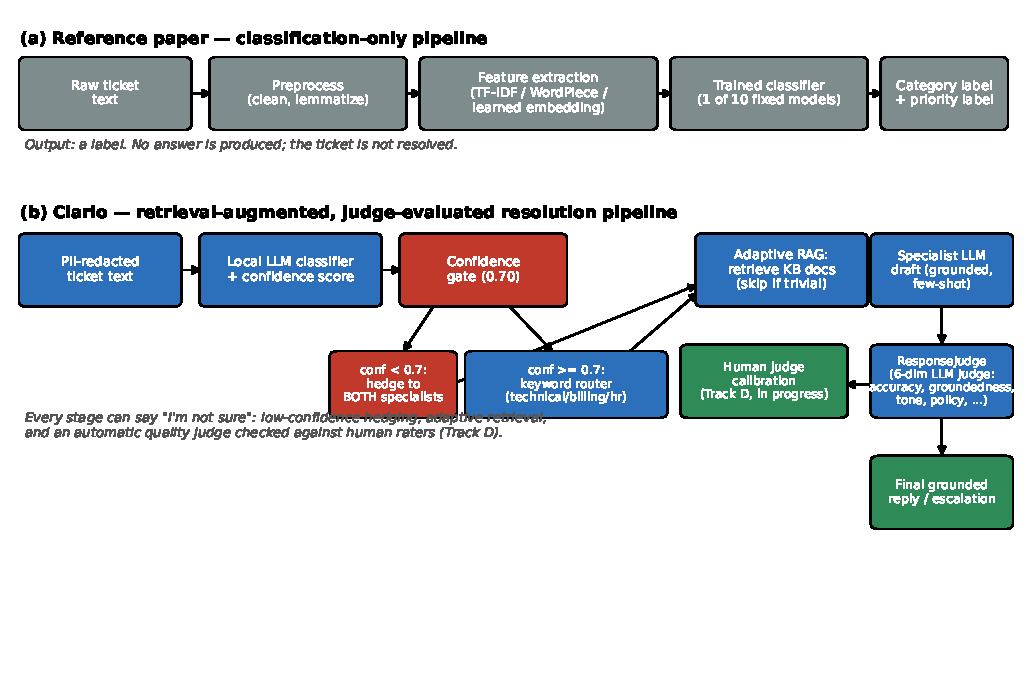
\includegraphics[width=0.92\textwidth]{figures/fig4_architecture.pdf}
\caption{Pipeline comparison. (a) The reference paper's pipeline ends at a label: a fixed, pre-trained model commits to one category and one priority, with no mechanism to express uncertainty or produce an answer. (b) Clario's pipeline treats classification as one signal among several, hedges under low confidence instead of forcing a guess, retrieves grounding evidence, generates a reply, and scores its own output against a judge that is itself checked against human raters.}
\label{fig:architecture}
\end{figure*}

\subsection{Confidence-Gated Classification}
Clario classifies a redacted ticket with a local LLM rather than a trained discriminative classifier, and reports a calibrated confidence score alongside the category, priority, and sentiment: the sequence-level confidence is computed as the softmax probability of each generated token, averaged across the generated sequence (mean of the chosen token's own probability at each decoding step). This is a materially different signal from a discriminative classifier's arg-max output: it is a property of \emph{how} the answer was generated, not just what the answer was.

\subsection{Routing That Can Say ``I Don't Know''}
The router (Section \ref{sec:methodology-clario}, \texttt{routing\_node}) does not trust the classifier's category label unconditionally. If classification confidence is below 0.70, or no category was produced at all, the ticket is routed to \emph{both} the technical and billing specialists rather than forced into one --- a direct, engineered response to the fact that a forced single-label classifier has no way to express ``I'm not sure which of these two this is.'' Above that threshold, the ticket is scored against small weighted-keyword tables (technical, billing, HR hard-triggers, HR weak-signals) that were tuned against real misrouting cases; for example, HR hard-trigger phrases (``medical'', ``parental consent'', ``bank slip'') route to HR even against competing billing signal, because that must-beat-everything requirement was measured to misroute 7 of 10 realistic HR tickets under an earlier, stricter rule. A one-time reroute flip exists if the first routing decision turns out to be wrong downstream. Retrieval itself is adaptive: very short queries (fewer than 5 words) skip the retrieval-augmented generation step entirely, since a greeting or a one-line message has no knowledge-base document to retrieve.

\subsection{Retrieval, Generation, and Judging}
For tickets that need it, Clario retrieves supporting knowledge-base documents, and a domain specialist LLM drafts a reply grounded in those documents using few-shot examples. \texttt{ResponseJudge}, an LLM-as-judge, then scores the draft on six dimensions --- overall quality, priority/tone match, completeness, accuracy, policy compliance, and groundedness --- each on a 1--5 scale. Unlike the reference paper's pipeline, every one of these stages produces an artifact that can be measured independently: the retrieval step has its own metrics (Section \ref{sec:results}), and the judge's own reliability is itself evaluated against human raters (Section \ref{sec:trackd}) rather than trusted by construction.

\section{Experimental Setup}
\label{sec:setup}

Two independent evaluation efforts are reported here.

\textbf{Classification reproduction} (Section \ref{sec:methodology-paper}): 20 models trained and evaluated on an 80/20 stratified split (16,000 train / 4,000 test), \texttt{random\_state=42} throughout, weighted precision/recall/F1/accuracy reported per the paper's own convention.

\textbf{Clario retrieval quality (``Track A'')}: does Clario's retrieval subsystem find the correct knowledge-base document for a ticket? Measured with Precision@$k$, Recall@$k$, Mean Reciprocal Rank, and nDCG@$k$ \cite{jarvelin2002ndcg}, leading with Precision@1 (was the top result right?) and Recall@4 (is the right document present at all in what production actually retrieves --- $k$=4). Ground truth was built by two annotators independently reading all 70 real tickets and each deciding the correct domain and document; disagreements (23 of 70) were resolved by taking the \emph{union} of both annotators' answers rather than picking one side, which is why some ground-truth entries name more than one correct domain. The two annotators agreed on at least one value 85.7\% of the time, and matched exactly 67.1\% of the time.

\textbf{Clario judge reliability (``Track D'', in progress)}: does \texttt{ResponseJudge}'s automatic score agree with a real person's judgment of the same reply? Methodology follows ARES \cite{saadfalcon2024ares}: draft replies and judge scores were generated for all 70 real tickets (bypassing the classifier/router so the sample is not biased by routing failures --- a separate, real Track B finding described in Section \ref{sec:trackd}), a stratified 28-pair sample was drawn for two independent human raters, and weighted Cohen's $\kappa$ \cite{cohen1960kappa} will be computed once both human scoring passes are complete.

\section{Results}
\label{sec:results}

\subsection{Classification Reproduction}
\label{sec:results-classification}

Figure \ref{fig:category-acc} and Table \ref{tab:leaderboard} show our reproduction's results. Every one of the 10 models clears 88\% accuracy on category classification, and the top four are within 1.6 points of each other. BERT wins both tasks (95.35\% category, 61.15\% priority), but a 1.3M-parameter BiLSTM reaches 95.00\% on category after roughly 70 seconds of training --- within 0.35 points of a 108M-parameter transformer that needed GPU fine-tuning. Priority classification is a materially harder problem for every model: the best result (BERT, 61.15\%) is only 19.8 points above the 41.4\% majority-class baseline, and every confusion matrix shows errors concentrated on \emph{adjacent} severity levels (Low$\leftrightarrow$Medium, Medium$\leftrightarrow$High) with almost no Low$\leftrightarrow$Urgent confusion --- the models learn the ordinal structure but cannot resolve neighboring boundaries from text alone.

\begin{figure}[t]
\centering
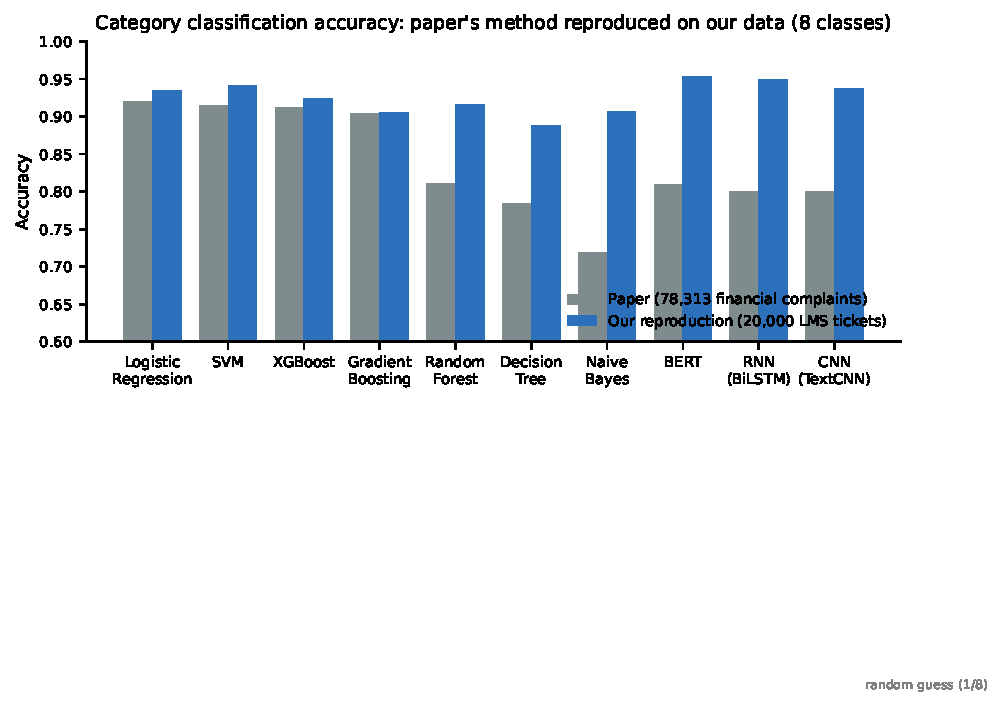
\includegraphics[width=\linewidth]{figures/fig1_category_accuracy.pdf}
\caption{Category classification accuracy: the paper's own reported numbers vs.\ the same 10 models trained on our data. Every model improves; see Section \ref{sec:discussion} for why this is a label-quality effect, not evidence of a better pipeline.}
\label{fig:category-acc}
\end{figure}

\begin{table}[t]
\centering
\caption{Overall leaderboard, our reproduction (mean of category and priority accuracy)}
\label{tab:leaderboard}
\begin{tabular}{@{}lccc@{}}
\toprule
Model & Category Acc. & Priority Acc. & Mean \\
\midrule
BERT & \textbf{0.9535} & \textbf{0.6115} & \textbf{0.7825} \\
RNN (BiLSTM) & 0.9500 & 0.5785 & 0.7643 \\
SVM & 0.9418 & 0.5823 & 0.7620 \\
Logistic Regression & 0.9348 & 0.5808 & 0.7578 \\
CNN (TextCNN) & 0.9375 & 0.5608 & 0.7491 \\
XGBoost & 0.9238 & 0.5590 & 0.7414 \\
Naive Bayes & 0.9070 & 0.5650 & 0.7360 \\
Random Forest & 0.9163 & 0.5548 & 0.7355 \\
Gradient Boosting & 0.9060 & 0.5303 & 0.7181 \\
Decision Tree & 0.8885 & 0.4865 & 0.6875 \\
\bottomrule
\end{tabular}
\end{table}

\subsection{Clario Retrieval Quality}
\label{sec:results-retrieval}

Figure \ref{fig:retrieval} shows the before/after picture on Clario's retrieval subsystem. The first evaluation (99 held-out queries) found the correct document \emph{somewhere} in the results 70.3\% of the time (Recall@4), but ranked it first only 20.3\% of the time (Precision@4) --- root-caused to stale content sitting in the search index and a relevance-confidence check that never once declined to answer. After removing the stale index content, retuning that confidence threshold, and adding natural customer-facing wording to the knowledge base, the same 99-query set improved to Recall@4 = 86.4\%, Precision@1 = 64.4\%. On an independently built set of 70 real tickets, the numbers are higher still (Recall@4 = 89.0\%, Precision@1 = 71.4\%), though we report honestly that part of that gap is because some knowledge-base wording was written with direct knowledge of that specific ticket population --- the 99-query number, built completely separately, is the more conservative estimate of how the system performs on ticket phrasing it has not effectively seen before.

\begin{figure}[t]
\centering
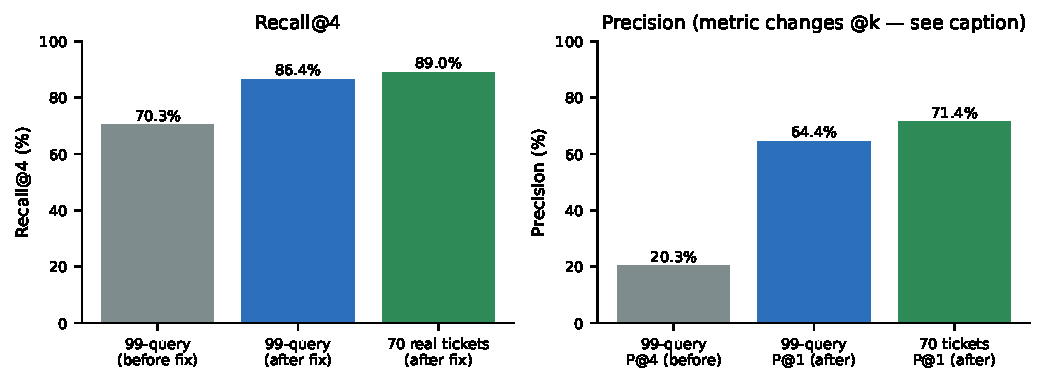
\includegraphics[width=\linewidth]{figures/fig3_retrieval_quality.pdf}
\caption{Clario retrieval quality before and after a diagnosed fix (stale index content removed, relevance-confidence threshold retuned). Precision is reported at different $k$ between rounds ($k$=4 before, $k$=1 after) and is labeled accordingly rather than implied to be like-for-like.}
\label{fig:retrieval}
\end{figure}

\section{Comparative Discussion}
\label{sec:discussion}

\subsection{Category Classification: A Real Improvement, With a Caveat}
Every one of the 10 models beats the paper's own reported accuracy on category classification (Table \ref{tab:cat-comparison}), several by more than 10 points. The most plausible explanation is not that our pipeline is better engineered; it is that our labels are better. The paper's category labels are \emph{derived} --- induced via NMF topic modeling and hand-mapped from the top-10 words of each topic into 5 departments --- which is a noisy, overlapping labeling process by construction. Ours are clean, pre-existing gold labels on data whose category was fixed at generation time. Read that way, our numbers are an \emph{upper bound} on what this style of classifier can do under clean labels, not proof our TF-IDF pipeline or our BERT fine-tuning recipe is superior to theirs.

\begin{table}[t]
\centering
\caption{Category accuracy: paper vs.\ our reproduction (full detail in Fig.~\ref{fig:category-acc})}
\label{tab:cat-comparison}
\small
\begin{tabular}{@{}lrrr@{}}
\toprule
Model & Paper & Ours & $\Delta$ \\
\midrule
Multinomial NB & 0.7187 & 0.9070 & \textbf{+18.8} \\
BERT & 0.81 & 0.9535 & \textbf{+14.4} \\
RNN & 0.80 & 0.9500 & \textbf{+15.0} \\
Decision Tree & 0.7844 & 0.8885 & \textbf{+10.4} \\
Random Forest & 0.8113 & 0.9163 & \textbf{+10.5} \\
SVM & 0.9151 & 0.9418 & +2.7 \\
Logistic Regression & 0.9199 & 0.9348 & +1.5 \\
\bottomrule
\end{tabular}
\end{table}

\subsection{Priority Classification: The Paper's Numbers Are a Warning, Not a Target}
Figure \ref{fig:priority-acc} makes the more important point. The paper reports up to 99.96\% accuracy (Decision Tree) and 99.73\% (XGBoost) on its binary urgent/not-urgent task, with precision and recall both reported at 1.00. Near-perfect scores on a free-text classification task are a target-leakage signature: the paper's priority labels were generated by keyword and negation matching over the \emph{same} ticket text the models then read, so a decision tree given TF-IDF features is not predicting urgency, it is reverse-engineering the labeling script. Our 4-class ordinal priority labels carry no such shortcut, and our 48--61\% range is a genuinely hard problem measured honestly. The two sets of numbers in Figure \ref{fig:priority-acc} are not measuring the same thing, and we say so directly in the figure rather than letting the visual similarity of two bar charts imply otherwise.

\begin{figure}[t]
\centering
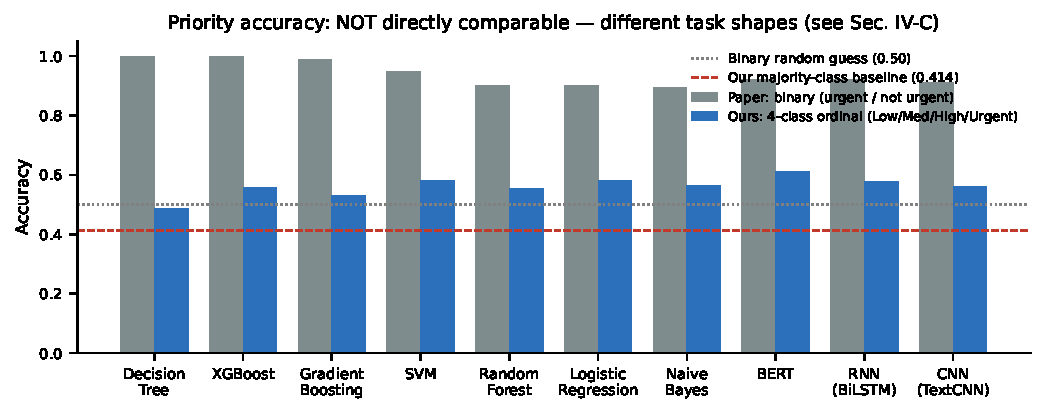
\includegraphics[width=\linewidth]{figures/fig2_priority_accuracy.pdf}
\caption{Priority accuracy, paper (binary, keyword-derived labels) vs.\ ours (4-class ordinal, gold labels). The paper's near-ceiling scores are consistent with target leakage from its own labeling method, not a harder problem solved better.}
\label{fig:priority-acc}
\end{figure}

This matters directly for the architecture question this paper is asking. If priority genuinely cannot be resolved from ticket text alone with confidence --- and both our honest 4-class numbers and the paper's leakage-inflated binary numbers are consistent with that --- then a production system that forces a single trained priority classifier into a hard routing decision is building on a foundation that either overfits to a labeling shortcut (the paper's approach) or is simply wrong close to 40\% of the time (our honest reproduction). Clario sidesteps this by using priority primarily to set the \emph{tone} of a generated reply, with a confidence-gated classifier and a human-in-the-loop escalation path for cases the router itself cannot resolve, rather than making the whole system's downstream behavior depend on one brittle classification.

\subsection{Class Imbalance: A Configuration Choice, Not an Architecture Choice}
One structural finding of the reproduction generalizes directly to system design. The three DL models applied balanced class weights to the priority task; the seven classical models did not. On the Urgent class (7.3\% of the data), the unweighted models buy high precision by almost never predicting Urgent --- Multinomial Naive Bayes finds only 60 of 291 urgent tickets (21\% recall) at 88\% precision --- while the weighted DL models trade some precision for 59--67\% Urgent recall. For a ticket-triage system, missing four out of five urgent tickets is the failure mode that actually matters. This is not a property of model family; it is a configuration choice available to any of the ten models. We flag it because it is exactly the kind of choice that is easy to get quietly wrong in a fixed, one-shot trained pipeline, and easy to catch when a system is instrumented and measured end to end the way Clario's retrieval subsystem was in Section \ref{sec:results-retrieval}.

\subsection{What the Reference Paper's Methodology Cannot Measure}
The comparison in Table \ref{tab:cat-comparison} and Figure \ref{fig:priority-acc} is, by construction, a comparison of classifiers. It says nothing about whether a customer's actual question gets answered, because the paper's pipeline stops at a label. There is no retrieval step to measure Precision@$k$ or Recall@$k$ on, no generated answer to check for groundedness, and no mechanism by which the system could say ``I don't have enough information to answer this.'' Section \ref{sec:results-retrieval}'s 70.3\%\,$\rightarrow$\,89.0\% Recall@4 improvement, and the diagnosed root causes behind it (stale index content, a confidence gate that never triggered), are only possible to report because Clario's architecture has a retrieval stage with its own measurable output. A classification-only system has no analogous lever to pull, because it has no analogous stage.

\subsection{A Shared Risk: Visible Automation Can Erode Trust}
\label{sec:trust-risk}
The architectural case made throughout this section should not be read as a claim that more automation is unconditionally better. Fuchs et al. \cite{fuchs2022} --- part of the same ML-bottleneck literature Hampel's platform survey \cite{hampel2024} discusses --- report that customer satisfaction measurably decreased once it became obvious to a customer that a chatbot, rather than a human agent, was handling their request, independent of whether the chatbot's answer was actually correct. This risk applies to Clario exactly as it would to any automated resolution system, and neither evaluation in this paper measures it: Track A (Section \ref{sec:results-retrieval}) measures whether the right document was retrieved, and Track D (Section \ref{sec:trackd}) measures whether a reply's content is good, but neither measures whether a customer's trust in the interaction is affected by knowing it was AI-generated in the first place. We flag this here rather than let Section \ref{sec:which-approach} imply automation is free of downside: a system that resolves tickets more accurately than a human-operated queue can still perform worse on end-to-end customer satisfaction if the fact of automation is poorly disclosed or handled. This is a genuine open question for Clario's roadmap (Section \ref{sec:future-work}), not a solved problem.

\section{Judge Reliability: An Honest Progress Report}
\label{sec:trackd}

Track D asks a narrower but important question: does \texttt{ResponseJudge}'s automatic score of a draft reply actually agree with what a human would say about the same reply? This evaluation is not yet complete --- both human scoring passes are pending as of this writing --- but generating the input data itself surfaced a real, actionable finding, which we report here rather than holding until the full $\kappa$ analysis is done.

Draft generation intentionally bypassed the classifier and router (a real Track B finding on its own: a smoke test showed the production classifier and keyword router escalate most of these 70 tickets before any specialist runs, because the classifier's generic category outputs do not match the router's keyword rules) and instead called the correct specialist directly using Track A's already-verified ground-truth domain, so that Track D's narrower question --- does the judge agree with a human? --- is not confounded by a separate, already-known routing problem.

Figure \ref{fig:judge-scores} shows what came back: \texttt{judge\_overall\_score} was exactly 2 out of 5 for 67 of 70 drafts (96\%), with \texttt{priority\_tone\_match\_score} (64/70) and \texttt{policy\_compliance\_score} (52/70) showing the same clustering, while \texttt{accuracy\_score} and \texttt{groundedness\_score} did not. We checked the root cause directly rather than assuming it was noise: the specialist's own draft-writing prompt never references \texttt{ResponseJudge}'s per-priority required-phrase checklist (for example, a Medium-priority reply is expected to include phrases like an apology for the inconvenience and a stated update window). The specialist has no way to write toward a rubric it was never shown, so nearly every draft is marked down for the same reason regardless of the quality of its actual troubleshooting content.

\begin{figure}[t]
\centering
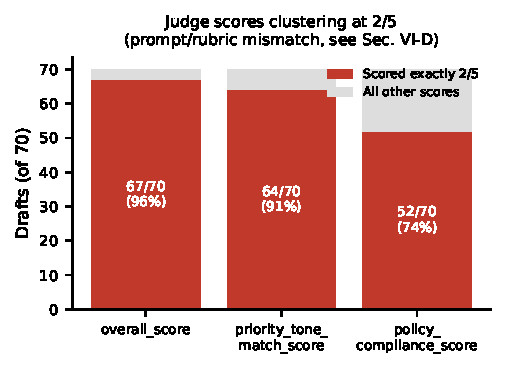
\includegraphics[width=\linewidth]{figures/fig5_judge_scores.pdf}
\caption{Judge scores clustering at 2/5 across three of six scoring dimensions, traced to a prompt/rubric mismatch: the draft-generation prompt does not expose the judge's required-phrase checklist.}
\label{fig:judge-scores}
\end{figure}

We report this as a limitation, not a success, but it is also a direct illustration of the architectural argument in Section \ref{sec:discussion}: this is a bug that a judge-evaluated pipeline can \emph{find}, because the judge produces an independently inspectable score per dimension. A classification-only pipeline has no equivalent surface on which a mismatch like this could even be observed. With scores this tightly clustered, \texttt{overall\_score} itself has little remaining variance for a $\kappa$ comparison to be informative about; \texttt{accuracy\_score} and \texttt{groundedness\_score}, which did not cluster, are expected to carry the real signal once both human scoring passes are complete. We note plainly, following ARES's own guidance \cite{saadfalcon2024ares}, that a 28-pair sample supports a general statement about judge/human agreement, not a tight confidence interval --- ARES's own benchmark used roughly 150 pairs for this purpose.

\section{Which Approach Fits a Ticket-Issuing System?}
\label{sec:which-approach}

Bringing the two evaluations together: for a system whose job is to \emph{categorize} tickets against clean, already-labeled data, the reference paper's methodology works well, and several of its lighter classical models (SVM, Logistic Regression) are a genuinely reasonable choice --- SVM lands third overall on our leaderboard (Table \ref{tab:leaderboard}) with no GPU and seconds of training, within 1.2 points of BERT on category. That is a fair, evidence-backed use case for the classification-only approach, and we do not overstate the case against it.

But a ticket-\emph{issuing} system, in the sense the user asked about, has to do more than route a ticket to the right queue: it has to produce an answer, know when it does not have enough information to produce one, and have a way to check whether that answer was actually good. None of the ten models evaluated in Sections \ref{sec:methodology-paper} and \ref{sec:results-classification} do any of that, by design --- they were never built to. Clario's architecture is built specifically for that harder problem: a confidence-gated classifier that hedges instead of guessing, a router with an explicit escalation path, retrieval that is measured and demonstrably improvable (Section \ref{sec:results-retrieval}), and a judge that checks its own output and is itself checked against humans (Section \ref{sec:trackd}). The evidence in this paper does not show Clario's classifier is more accurate than a fine-tuned BERT --- it isn't trying to be one. It shows that accuracy on a label is the wrong axis to evaluate a resolution system on, and that the axes which matter for resolution (grounded retrieval, hedged routing, self-checked generation) are exactly the ones the classification-only methodology has no way to produce or measure.

This is not only true of the ten classifiers reproduced in this paper; it is true of the ticketing systems actually deployed in industry today. Hampel's independent, hands-on evaluation of five widely used commercial and open-source platforms \cite{hampel2024} found that none of them retrieve grounding evidence, draft a reply, or evaluate their own output --- Table \ref{tab:market-comparison} summarizes the gap. Where AI-driven automation exists at all in that survey (Jira, Zendesk), it is a paywalled add-on layered onto a rule-based workflow engine, not an architectural first-class citizen the way retrieval, generation, and judging are in Clario. This corroborates, from an independent source, that the resolution capability evaluated in this paper is not yet standard in the market Clario operates in.

\begin{table}[t]
\centering
\caption{Automation capability: five deployed platforms \cite{hampel2024} vs.\ Clario. ``Add-on'' = AI automation exists only as a paywalled or third-party layer, not a first-party architectural stage.}
\label{tab:market-comparison}
\small
\begin{tabular}{@{}lccc@{}}
\toprule
System & AI-native & Grounded & Self- \\
 & automation & answer & evaluated \\
\midrule
Jira & Add-on & No & No \\
Zendesk & Add-on & No & No \\
Znuny/OTRS & No & No & No \\
GitLab & No & No & No \\
Trac & No & No & No \\
\textbf{Clario} & \textbf{Yes} & \textbf{Yes} & \textbf{Yes} \\
\bottomrule
\end{tabular}
\end{table}

We take this as further support, not as the core of the argument: even if a reader remains unconvinced that classifier accuracy is the wrong axis, the market evidence in Table \ref{tab:market-comparison} shows that grounded, self-checking automation of the kind Clario provides is not something a support team can simply buy off the shelf by picking a more automated ticketing platform. It has to be built the way Clario builds it --- as an architecture, not a feature toggle. (Section \ref{sec:trust-risk} notes an important boundary on this advantage: automation itself is not risk-free, per Fuchs et al. \cite{fuchs2022}.)

\section{Limitations and Threats to Validity}
\label{sec:limitations}

We report these directly rather than deferring them to future work, following the standard this evaluation effort has held throughout \cite{ds-eval-proposal}.

\begin{itemize}
\item \textbf{Synthetic classification data.} Our 20,000-ticket dataset is Gemini-generated, not real customer text. Both custom vocabularies (RNN/CNN) converged near 2,080 tokens against a 20,000-token cap, indicating unusually narrow, template-like language. Our classification numbers should be read as an upper bound on real-world performance, not a direct estimate of it.
\item \textbf{Priority task shapes are not comparable.} The paper's priority task is binary; ours is 4-class ordinal. Figure \ref{fig:priority-acc} and Table \ref{tab:leaderboard} report both, clearly labeled, but they are not a like-for-like accuracy comparison, and we do not treat them as one.
\item \textbf{TF-IDF fitted before the split.} Our classical ML reproduction fits TF-IDF on the full corpus before the train/test split, a mild optimistic bias absent from the RNN/CNN vocabularies (fitted on the training split only).
\item \textbf{No validation split, no early stopping.} All 20 reproduced models overfit visibly on the priority task (e.g., BERT reaches 0.046 training loss at 61\% test accuracy); this matches the paper's own undocumented validation protocol but is a real weakness in both.
\item \textbf{Track D is incomplete.} The judge-reliability $\kappa$ analysis requires both human scoring passes, which had not been completed at the time of writing. The prompt/rubric finding in Section \ref{sec:trackd} is real and actionable regardless, but the quantitative agreement claim is future work, not a result of this paper.
\item \textbf{Track A's higher real-ticket score is partly self-referential.} Some knowledge-base wording was written with direct knowledge of the 70-ticket evaluation set; the independently built 99-query set (Recall@4 86.4\%, Precision@1 64.4\%) is the more conservative estimate and the one we recommend planning around.
\item \textbf{Small human-calibration sample.} 28 judge/human pairs (Track D) supports a general statement about agreement, not a tight interval, consistent with ARES's own guidance \cite{saadfalcon2024ares}.
\end{itemize}

\section{Future Work}
\label{sec:future-work}
Three efforts are already in motion and were deliberately excluded from this paper's claims until they are complete: (1) finishing Track D's human scoring and computing weighted Cohen's $\kappa$ for judge/human and human/human agreement; (2) Track B, which will formally measure the routing/escalation accuracy problem this paper's Track D setup had to work around; and (3) fixing the specialist prompt to expose \texttt{ResponseJudge}'s required-phrase checklist directly, then re-running Track D to check whether the score clustering in Figure \ref{fig:judge-scores} resolves. We also intend to test whether the dataset's currently unused \texttt{issue\_complexity\_score} and \texttt{sentiment} fields improve priority classification, since both the paper's leakage-inflated numbers and our own honest ones point at the same conclusion: priority is not fully resolvable from ticket text alone.

\section{Conclusion}
We reproduced a published ticket-classification methodology on our own data and beat its reported accuracy on every one of ten models, but showed that the gap is best explained by label quality, not modeling superiority, and that the paper's own priority numbers carry a clear target-leakage signature. Separately, we evaluated Clario, a production system that treats classification as one signal inside a larger, retrieval-augmented, self-checking pipeline, and showed that its retrieval subsystem was measured, diagnosed, and demonstrably improved (Recall@4 70.3\%\,$\rightarrow$\,89.0\%) using a methodology that has no equivalent in a classification-only architecture, because that architecture has no retrieval or generation stage to measure in the first place. For a system whose job is only to sort tickets into bins against clean labels, classical and deep classifiers remain a sound, well-understood choice. For a system whose job is to resolve a ticket --- find the right knowledge, write a grounded answer, and know when it cannot --- the evidence in this paper points toward Clario's architecture: not because its classifier is more accurate, but because it is built to measure, hedge, and correct the parts of the problem a label alone cannot address. This conclusion is reinforced by an independent, hands-on survey of five widely deployed commercial ticketing platforms \cite{hampel2024}: none of them retrieve grounding evidence, draft an answer, or evaluate their own output, confirming that the resolution capability evaluated in this paper is not yet standard in the market Clario operates in --- though, as Section \ref{sec:trust-risk} makes clear via Fuchs et al. \cite{fuchs2022}, that capability is not a risk-free substitute for a human agent either. We have reported this work, including its unresolved parts, as it stands today; the judge-reliability and routing-accuracy tracks referenced throughout are ongoing and will be reported as they complete.

\begin{thebibliography}{00}
\bibitem{selvi2025} C. S. Kanimozhi Selvi, S. Jyothi Shri, R. Prasshanthini, Neelamegan, and R. Sanjay, ``Customer Support Ticket Categorization and Prioritization Using Natural Language Processing,'' Department of Artificial Intelligence, Kongu Engineering College, Erode, Tamil Nadu, India, presented at INCOFT 2025.
\bibitem{lewis2020rag} P. Lewis et al., ``Retrieval-Augmented Generation for Knowledge-Intensive NLP Tasks,'' in \emph{Advances in Neural Information Processing Systems (NeurIPS)}, 2020.
\bibitem{saadfalcon2024ares} J. Saad-Falcon, O. Khattab, C. Potts, and M. Zaharia, ``ARES: An Automated Evaluation Framework for Retrieval-Augmented Generation Systems,'' arXiv:2311.09476, 2024.
\bibitem{zheng2023judging} L. Zheng et al., ``Judging LLM-as-a-Judge with MT-Bench and Chatbot Arena,'' in \emph{Advances in Neural Information Processing Systems (NeurIPS)}, 2023.
\bibitem{jarvelin2002ndcg} K. J{\"a}rvelin and J. Kek{\"a}l{\"a}inen, ``Cumulated Gain-Based Evaluation of IR Techniques,'' \emph{ACM Transactions on Information Systems}, vol. 20, no. 4, pp. 422--446, 2002.
\bibitem{kim2014textcnn} Y. Kim, ``Convolutional Neural Networks for Sentence Classification,'' in \emph{Proceedings of EMNLP}, 2014.
\bibitem{cohen1960kappa} J. Cohen, ``A Coefficient of Agreement for Nominal Scales,'' \emph{Educational and Psychological Measurement}, vol. 20, no. 1, pp. 37--46, 1960.
\bibitem{hampel2024} J. Hampel, ``An Evaluation of Ticketing Systems,'' Seminar Report, HPCSA course, Institute of Computer Science, Georg-August-Universit{\"a}t G{\"o}ttingen, supervised by S. M{\"u}hlhausen, J. Decker, and J. Kunkel, Mar. 2024.
\bibitem{jantti2012} M. J{\"a}ntti, ``Examining Challenges in IT Service Desk System and Processes: A Case Study,'' in \emph{Proc. Seventh International Conference on Systems (ICONS)}, 2012, pp. 105--108.
\bibitem{qamili2018} R. Qamili, S. Shabani, and J. Schneider, ``An Intelligent Framework for Issue Ticketing System Based on Machine Learning,'' in \emph{Proc. IEEE 22nd International Enterprise Distributed Object Computing Workshop (EDOCW)}, 2018, pp. 79--86.
\bibitem{montgomery2018escalation} L. Montgomery et al., ``Customer Support Ticket Escalation Prediction Using Feature Engineering,'' \emph{Requirements Engineering}, vol. 23, pp. 333--355, 2018.
\bibitem{fuchs2022} S. Fuchs, C. Drieschner, and H. Wittges, ``Improving Support Ticket Systems Using Machine Learning: A Literature Review,'' in \emph{Proc. 55th Hawaii International Conference on System Sciences (HICSS)}, 2022, pp. 1893--1902.
\bibitem{ds-eval-proposal} Clario Data Science Evaluation Proposal: Retrieval Quality, Routing Accuracy, Response Quality, Judge Reliability, and System Behaviour, internal technical report, 2026.
\end{thebibliography}

\end{document}
